\graphicspath{ {Figures/system_analysis/} }

\chapter{Ανάλυση και σχεδιασμός του συστήματος LifeDonor}\label{ch:Analysis of LifeDonor}
\section{Λειτουργικές απαιτήσεις}

	Οι απαιτήσεις ενός συστήματος αποτελούν τη βάση των συστημάτων λογισμικού. Ουσιαστικά, είναι η περιγραφή των υπηρεσιών που πρέπει να παρέχει ένα σύστημα λογισμικού και οι περιορισμοί υπό τους οποίους πρέπει αυτές να λειτουργούν. Διακρίνονται σε δύο βασικές κατηγορίες τις λειτουργικές απαιτήσεις (functional requirements) και τις μη λειτουργικές απαιτήσεις(non functional requirements). 
	
	Οι λειτουργικές απαιτήσεις προσδιορίζουν τα βασικά χαρακτηριστικά του συστήματος και την λειτουργία του από την άποψη του ίδιου του προϊόντος και των χρηστών του . Στον όρο λειτουργία του συστήματος συμπεριλαμβάνεται οι συνολικές είσοδοι, η συμπεριφορά και οι έξοδοι του συστήματος. Στο σύστημα που υλοποιούμε, οι λειτουργικές απαιτήσεις χρησιμοποιούνται για να περιγράψουν ειδικές λειτουργίες που καθορίζουν αυτά τα οποία αναμένουμε να πετύχει το σύστημα. Αν και αναφέρονται ως "απαιτήσεις", στην πραγματικότητα αποτελούν μια μορφή σχεδιασμού, υψηλού επιπέδου. Οι λειτουργικές απαιτήσεις συχνά προσδιορίζονται ως λειτουργικές προδιαγραφές,» και ο όρος περιγραφή αποτελεί συνώνυμο του σχεδιασμού. Οι λειτουργικές απαιτήσεις είναι ουσιαστικά το "τι" λειτουργία θέλουμε να επιτελεί το σύστημα, χωρίς να παρέχουμε καμία πληροφορία για το "πως".
	
	Οι μη λειτουργικές απαιτήσεις είναι οι απαιτήσεις που καθορίζουν τα κριτήρια που χρησιμοποιούνται για να κρίνουν την λειτουργία του συστήματος και κατ΄ επέκταση  αν είναι επιτυχημένο ή όχι, για αυτό και συχνά αποκαλούνται και ιδιότητες του. Επεξεργάζονται τα χαρακτηριστικά απόδοσης του, και μπορούν επίσης να περιγράψουν τις πτυχές του συστήματος που δεν σχετίζονται με την εκτέλεση του, αλλά με την εξέλιξη του στο πέρασμα του χρόνου. Οι βασικές συνήθεις κατηγορίες των μη λειτουργικών απαιτήσεων σχετίζονται με την ασφάλεια( ασφαλή πρόσβαση σε δεδομένα αλλά και σε hardware), την απόδοση ( ορίζουν χαρακτηριστικά που έχουν να κάνουν με την ταχύτητα και την ανταπόκριση του συστήματος) και την επεκτασιμότητα (σχετίζονται με το μέγεθος του συστήματος). Γενικότερα, οι μη λειτουργικές απαιτήσεις καθορίζουν το πώς πρέπει να είναι ένα σύστημα, σε αντίθεση με τις λειτουργικές απαιτήσεις που καθορίζουν τι πρέπει να κάνει ένα σύστημα. Οι λειτουργικές απαιτήσεις ανήκουν στο κομμάτι σχεδιασμού και ανάλυσης του συστήματος ενώ οι μη λειτουργικές απαιτήσεις ανήκουν στο κομμάτι της αρχιτεκτονικής του συστήματος.
	
	\subsection{Λειτουργίες εφαρμογής (web, mobile)}
Οι χρήστες του συστήματος χωρίζονται σε τρεις μεγάλες ομάδες χρηστών.
		\begin{enumerate}
			\item Εθελοντές αιμοδότες
			\item Εγκεκριμένοι χρήστες/διαχειριστές των συστημάτων αιμοδοσίας
			\item Υπέρ-Διαχειριστές του συστήματος
		\end{enumerate}
		
		Οι εθελοντές αιμοδότες αποτελούν την βασική κατηγορία χρηστών καθώς πραγματοποιούν συνεχή και εκτεταμένη χρήση των υπηρεσιών του συστήματος, τόσο στο επίπεδο της εφαρμογής έξυπνου κινητού όσο και μέσω του web portal. Οι εγκεκριμένοι χρήστες/διαχειριστές των συστημάτων αιμοδοσίας χρησιμοποιούν αποκλειστικά το web portal το οποίο βρίσκεται στο υπολογιστικό νέφος για ολοκληρωμένη διαχείριση ενός πλήρη κύκλου αιμοδοσίας Οι λειτουργίες που μπορεί να επιτελέσει κάθε ομάδα χρηστών καθώς και οι λειτουργικές απαιτήσεις του συστήματος αναλύονται με λεπτομέρειες στην συνέχεια.
		\subsubsection{Mobile} \label{sssec:functional_requirements_mobile}
			Περιληπτικά (θα αναλυθούν με λεπτομέρειες στην συνέχεια) οι λειτουργικές απαιτήσεις της εφαρμογής έξυπνου κινητού έχουν ως εξής:
			\begin{itemize}
				\item Δυνατότητα εγγραφής στο σύστημα ως εθελοντής αιμοδότης με χρήση του αριθμού μητρώου κοινωνικής ασφάλισης (Α.Μ.Κ.Α.).
				\item Δυνατότητα σύνδεσης στο σύστημα αν έχει πραγματοποιήσει ήδη έγγραφή στο παρελθόν.
				\item Δυνατότητα προβολής γεγονότων αιμοδοσίας.
				\item Δυνατότητα λήψης ειδοποιήσεων (push notifications) όταν δημιουργείται κάποιο νέο γεγονός αιμοδοσίας για το οποίο ο εθελοντής αιμοδότης πληρεί τα απαραίτητα κριτήρια.
				\item Δυνατότητα αποδοχής, απόρριψης ή αναβολής της ειδοποίησης για το γεγονός αιμοδοσίας.
				\item Δυνατότητα διαχείρισης ραντεβού για αιμοδοσία (δημιουργία νέου ραντεβού, μετάθεση , προβολή, ακύρωση).
				\item Δυνατότητα προσθήκης και συγχρονισμού των ραντεβού αιμοδοσίας στο ημερολογίου του χρήστη.
				\item Δυνατότητα ενημέρωσης σχετικά με το υπολειπόμενο διάστημα που πρέπει να παρέλθει ώστε ο εθελοντής να είναι σε θέση να συμμετέχει σε μία νέα αιμοδοσία.
				\item Δυνατότητα να κερδίσει πόντους και εμβλήματα βάση των αιμοδοσιών του (gamification system) και να τα μοιραστεί στα μέσα κοινωνικής δικτύωσης.
				\item Δυνατότητα να μοιραστεί και να δημοσιεύσει στοιχεία στα μέσα κοινωνικής δικτύωσης σε κάθε στάδιο της αιμοδοσίας.
				\item Δυνατότητα δημιουργίας έκκλησης για αίμα σε περίπτωση ανάγκης ατόμων του στενού κύκλου χρήστη και δημοσίευσης του στα μέσα κοινωνικής δικτύωσης.
				\item Δυνατότητα διαχείρισης προφίλ χρήστη.
			\end{itemize}
			\subsubsection{Web Portal} \label{sssec:functional_requirements_web}
				Το web portal που βρίσκεται στο υπολογιστικό νέφος χρησιμοποιείται απο όλες τις ομάδες χρηστών. Όσον αφορά στους εθελοντές αιμοδότες ισχύουν οι ίδιες λειτουργικές απαιτήσεις όπως στην εφαρμογή του έξυπνου κινητού οι οποίες και αναλύθηκαν παραπάνω στο \ref{sssec:functional_requirements_mobile}. Όσον αφορά στους χρήστες/διαχειριστές των κέντρων αιμοδοσίας έχουμε τις παρακάτω λειτουργικές απαιτήσεις:
				\begin{itemize}
					\item Δημιουργία νέων γεγονότων αιμοδοσίας.
					\item Αποστολή ειδοποιήσεων στους εθελοντές αιμοδότες βάση των γεγονότων αιμοδοσίας, των αναγκών και των κριτηρίων αποδοχής.
					\item Προβολή στατιστικών ανά έτος σχετικά με τις ειδοποιήσεις που στάλθηκαν από το συγκεκριμένο κέντρο αιμοδοσίας και την ανταπόκριση των χρηστών (αποδοχή, απόρριψη, άνοιγμα ειδοποίησης, ολοκλήρωση αιμοδοσίας).
					\item Διαχείριση των ραντεβού για αιμοληψία.
					\item Διαχείριση του προφίλ του κέντρου αιμοδοσίας.
				%	\item Εισαγωγή δεδομένων από το τοπικό τους σύστημα στο κεντρικό σύστημα μας που βρίσκεται στο υπολογιστικό νέφος
					\item Δυνατότητα εγγραφής στο σύστημα νέου εθελοντή αιμοδότη.
					\item Δυνατότητα καταχώρησης της ολοκλήρωσης της αιμοδοσίας.
					\item Δυνατότητα ελέγχου τήρησης προϋποθέσεων καταλληλότητας εθελοντή αιμοδότη.
				\end{itemize}
				Όσον αφορά στους υπέρ-διαχειριστές του συστήματος έχουμε τις παρακάτω λειτουργικές απαιτήσεις:
				\begin{itemize}
					\item Δυνατότητα διαχείρισης λογαριασμών χρηστών.
					\item Προβολή στατιστικών για τους χρήστες του συστήματος.
				\end{itemize}

	\subsection{Social Networking Integration}
	\subsection{Gamification}
		Το gamification (παιχνιδοποιήση) ορίζεται ως "η ενσωμάτωση διάφορων πρακτικών και διαδικασιών παιχνιδιού σε καταστάσεις που δεν σχετίζονται με το παιχνίδι με στόχο τη λύση προβλημάτων μέσω της αύξησης της διαδραστικότητας και της συμμετοχής των χρηστών"\cite{Deterding:2011:GDE:2181037.2181040}\cite{Rojas:2013:MPG:2583008.2583033}. Ως εκ τούτου, το gamification έχει βρει χρήση σε ένα ευρύ φάσμα εφαρμογών, από τον χώρο του marketing και της εκπαίδευσης μέχρι και τον χώρο της υγείας \cite{6758978}. Το Gartner έχει εκτιμήσει ότι μέχρι το τέλος του 2015 περισσότερο από το 50\% των επιχειρήσεων θα αξιοποιεί το gamification \cite{gartnerGamification}. Στον ακαδημαϊκό χώρο συναντάμε όλο και περισσότερη έρευνα και δημοσιεύσεις με στόχο να μελετηθεί με μετρήσιμα, αντικειμενικά κριτήρια κατά πόσο είναι αποτελεσματική η χρήση των τεχνικών gamifaction. Ένα παιχνίδι αποτελείται από έξι δομικά στοιχεία, όπως παρουσιάζονται στο σχήμα \ref{fig:gamification_components}.
		
	\begin{figure}[h]
	    \centering
	    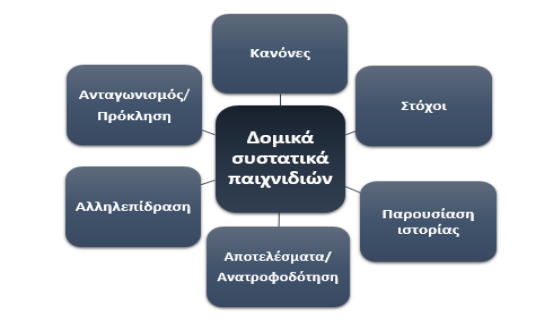
\includegraphics[width=0.7\textwidth]{gamification_components.jpg}
	    \caption{Δομικά στοιχεία παιχνιδιών}
	    \label{fig:gamification_components}
	\end{figure}
	
	Ένας από τους βασικούς στόχους ενός συστήματος gamification αποτελεί η αύξηση της ενασχόλησης του χρήστη. Τα στάδια με τα οποία ευελπιστεί να το πετύχει έχουν ως εξής:
	\begin{enumerate}
		\item Κίνητρα: Στην αρχή της διαδικασίας θα πρέπει να δοθεί στον χρήστη κάποιο κίνητρο το οποίο διαφέρει ανάλογα με τον τύπο χρήστη καθώς και τους στόχους του συστήματος. Παράδειγμα ενός τέτοιου κινήτρου αποτελεί η κοινωνική αναγνώριση \cite{Gamification_on_Participation}.
		\item Ενέργειες: είναι το δεύτερο στάδιο στο οποίο ο χρήστης οδηγείται μέσω των κινήτρων του πρώτου σταδίου. Σε αυτό το στάδιο ο χρήστης πραγματοποιεί την επιθυμητή από το σύστημα ενέργεια. Για παράδειγμα σε μια εφαρμογή εκμάθησης ξένων γλωσσών μια ενέργεια μπορεί να είναι η επανάληψη του λεξιλογίου.
		\item Επιβραβεύσεις: Ύστερα από την επιτυχή ολοκλήρωσης της ενέργειας ή των ενεργειών στο δεύτερο βήμα ο χρήστης λαμβάνει κάποια μορφή επιβράβευσης. Παραδείγματα επιβραβεύσεων που βρίσκουν ευρεία χρήση στο gamification αποτελούν τα εικονικά νομίσματα και τα εικονικά αγαθά.
		\item Κατορθώματα: Στο τελευταίο αυτό στάδιο ο χρήστης φτάνει σε κάποιο κατόρθωμα το οποίο ενισχύει τα κίνητρα του και ο κύκλος επαναλαμβάνεται \cite{GamificationDesign}.
	\end{enumerate}
	Η διαδικασία όπως την περιγράψαμε εμφανίζεται στο σχήμα \ref{fig:engagement_loop}.
	\begin{figure}[h]
	    \centering
	    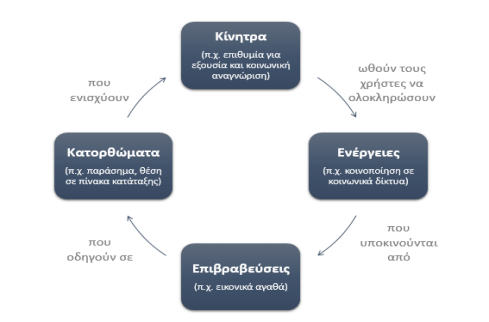
\includegraphics[width=0.7\textwidth]{engagement_loop.jpg}
	    \caption{Κύκλος ενασχόλησης}
	    \label{fig:engagement_loop}
	\end{figure}
\section{UML diagrams - Σενάρια χρήσης  }

	Η διαδικασία της μοντελοποίησης, δηλαδή ο αναλυτικός σχεδιασμός ενός συστήματος, πριν από την υλοποίηση του είναι ένα πολύ βασικό στάδιο κατά την ανάπτυξη εφαρμογών. Ένα σύστημα μοντελοποιείται επιτυχώς όταν οι λειτουργικότητες του συστήματος έχουν περιγραφεί πλήρως και ορθώς, έχουν καλυφθεί οι ανάγκες των τελικών χρηστών και υποστηρίζεται η επεκτασιμότητα του συστήματος. 
	Η ενοποιημένη Γλώσσα Μοντελοποίησης (UML) είναι μια τυπική γλώσσα για την σύνταξη λεπτομερών σχεδίων λογισμικού. Η UML μπορεί να χρησιμοποιηθεί για να απεικονίσει, να προσδιορίζει,να κατασκευάσει και να τεκμηριώσει τα προϊόντα του συστήματος εντάσεως λογισμικού.\cite{Booch2005}. Δεν αποτελεί απλώς έναν κατάλογο από διαγράμματα, αλλά είναι μια γλώσσα αναπαράστασης γνώσης. Αυτό συνεπάγεται ότι κάθε στοιχείο διαγράμματος, π.χ. κουτί, βέλος, κύκλος, ορθογώνιο κ.λπ., υποστηρίζεται από συγκεκριμένους κανόνες σύνταξης και σημασιολογία.
	 Επιλέξαμε να μοντελοποιήσουμε το σύστημα μας με χρήση της γλώσσας UML για τους εξής λόγους:
	 \begin{itemize}
	 \item Είναι ένα βιομηχανικό πρότυπο από τον διεθνή, ανοιχτό και μη κερδοσκοπικό οργανισμό εταιριών Object Management Group (OMG).
	 \item Η UML είναι χτισμένη πάνω σε θεμελιώσεις αντικειμενοστραφείς έννοιες, όπως η κλάση, με αποτέλεσμα να υποστηρίζει καλύτερα την ανάπτυξη και τον σχεδιασμό του αντικειμενοστραφούς λογισμικού.
	 \item Δίνει έμφαση στην ανάλυση των σεναρίων χρήσης, το οποίο είναι ένα πολύτιμο εργαλείο για την παρακολούθηση των σταδίων μιας διαδικασίας από την οπτική γωνία του χρήστη.
	 \item Δίνει στον σχεδιαστή την δυνατότητα να παρουσιάσει όσο λεπτομερώς επιθυμεί αυτός τις περιγραφές του συστήματος.
	 \item Τμηματοποιεί τον σχεδιασμό του συστήματος με αποτέλεσμα να αυξάνεται η επεκτασιμότητα του.
\end{itemize}	 

	Η UML 2.0 ορίζει δεκατρείς τύπους διαγραμμάτων, τα οποία μπορούν να χωριστούν σε δύο βασικές κατηγορίες:
	\begin{itemize}
		\item Τα διαγράμματα στατικής δομής, τα οποία δείχνουν τα πράγματα τα οποία απαρτίζουν το σύστημα που μοντελοποιείται και δεν αλλάζουν στο πέρασμα του χρόνου, για παράδειγμα τις κλάσεις, τα αντικείμενα κλπ. Στα διαγράμματα δομής ανήκουν : τα διαγράμματα κλάσεων, τα διαγράμματα αντικειμένων, τα ψηφιδικά διαγράμματα, τα διαγράμματα σύνθετης δομής, τα διαγράμματα πακέτου και τα διαγράμματα διάταξης.
		\item Τα διαγράμματα συμπεριφοράς, τα οποία δίνουν έμφαση στο τι πρέπει να γίνει στο σύστημα που μοντελοποιούμε, όπως τις αλληλεπιδράσεις με τους χρήστες, τις διάφορες καταστάσεις του συστήματος κλπ. Διαγράμματα συμπεριφοράς αποτελούν τα ακόλουθα: τα διαγράμματα χρήσης, τα διαγράμματα δραστηριότης, τα διαγράμματα καταστάσεων μηχανής, τα ακολουθιακά διαγράμματα, τα συνεργατικά διαγράμματα και τα διαγράμματα χρονισμού.
	\end{itemize}
Κάθε ένα από τα παραπάνω διαγράμματα βλέπει το σύστημα από μια διαφορετική οπτική γωνία, π.χ. τα διαγράμματα χρήσης δείχνουν πώς οι χρήστες αλληλεπιδρούν με το σύστημα, τα διαγράμματα κλάσης δείχνουν τις κλάσεις του συστήματος και τις σχέσεις μεταξύ τους κλπ.

	Στο πλαίσιο της διπλωματικής μας, θα χρησιμοποιήσουμε διαγράμματα χρήσης (use cases diagrams). Τα διαγράμματα χρήσης είναι τα διαγράμματα υψηλότερου επιπέδου της UML και αποτυπώνουν την συμπεριφορά του συστήματος από την σκοπιά ενός εξωτερικού χρήστη. Περιγράφονται όλες οι λειτουργίες του συστήματος σε έναν γραφικό πίνακα περιεχομένων (τι πρέπει να κάνει το σύστημα και όχι το πως θα το κάνει).  Τα διαγράμματα χρήσης έχουν τέσσερα βασικά συστατικά:
	
	\begin{itemize}
		\item Τους δράστες, που είναι χρήστες, ένας οργανισμός, εξωτερικά συστήματα κλπ..Κάθε δράστης συνδέεται με αρκετά σενάρια χρήσης καθένα από τα οποία περιγράφει τι θέλει να κάνει ο δράστης με το σύστημα.
		\item Τα σενάρια χρήσης ( τα οποία αναπαρίστανται με οβάλ σχήματα και το όνομα των σεναρίων ),  τα οποία περιγράφουν μία σειρά από πράξεις που πρέπει να εκτελεστούν για να επιτευχθεί ή να εγκαταλειφθεί ο στόχος του δράστη.
		\item Τις γραμμές που αντιπροσωπεύουν διάφορους τύπους σχέσεων (πχ isa, περιλαμβάνει, επεκτείνει κλπ) μεταξύ ενός δράστη και ενός σεναρίου χρήσης, μεταξύ δύο σεναρίων χρήσης και μεταξύ δύο δραστών. 
		\item Τα όρια του συστήματος που αντιπροσωπεύεται από ένα τετράγωνο που περιλαμβάνει όλα τα σενάρια χρήσης που υποδεικνύουν τις λειτουργικότητες του συστήματος. 

	\end{itemize}
	

Η πρακτική της ανάλυσης με σενάρια χρήσης τυποποιήθηκε για πρώτη φορά από τον Jacobson το 1994, ο οποίος περιέγραψε το σενάριο χρήσης σαν "μία σειρά από συναλλαγές που σχετίζονται ως προς την συμπεριφορά και εκτελούνται από έναν δράστη που βρίσκεται σε επικοινωνία με το σύστημα με σκοπό την παροχή κάποιας μετρήσιμης αξίας στον δράστη" \cite{Jacobson} . Ένα σενάριο χρήσης είναι μία συλλογή από πιθανά σενάρια μεταξύ του συστήματος και των εξωτερικών του δραστών. Κάθε σενάριο χρήσης χαρακτηρίζεται από τον στόχο που έχει ο κύριος δράστης του. Ο στόχος αυτός μπορεί να επιτευχθεί ή όχι. Τα σενάρια χρήσης αποτελούν ένα πολύ διαδεδομένο και πολύτιμο εργαλείο για την πλήρη αποτύπωση των λειτουργικών απαιτήσεων του συστήματος. Οι λειτουργικές απαιτήσεις μπορούν να εκφραστούν είτε με μορφή κειμένου, είτε με μορφή πίνακα. Επιλέξαμε να χρησιμοποιήσουμε την μορφή πίνακα, καθώς έχει πιο αυστηρή δομή με αποτέλεσμα να μειώνονται οι ασυνέπειες και οι περιττές πληροφορίες. \cite{Cockburn2000} και πιο συγκεκριμένα την μονή στήλη πρότυπο \cite{Cockburn2000} :
 
 Ο τίτλος του σεναρίου χρήσης, που συνήθως είναι ένα μία πρόταση που περιγράφει τον στόχο του κύρίως δράστη.
 Το πλαίσιο του στόχου
 Μία μεγαλύτερη δήλωση η οποία περιγράφει τον στόχο του σεναρίου χρήσης με περισσότερες λεπτομέρειες.
 Λεπτομέρειες
 Κύριοι δράστες: Είναι οι δράστες που έχουν ως στόχο αυτόν που περιγράφεται από το σενάριο χρήσης.
 Προϋποθέσεις: αυτά που ισχύουν πριν ξεκινησει να εκτελείται το σενάριο χρήσης. Εφόσον είναι γνωστό ότι μια συνθήκη είναι αληθής, δεν θα ελεγχθεί ξανά κατά την διάρκεια εκτέλεσης του σεναρίου χρήσης. 
 Επίπεδα: τα επίπεδο των στόχων είναι ένα από τα παρακάτω 
 \begin{itemize}
\item  Περίληψης:  Ένα περιληπτικού στόχου σενάριο χρήσης παρέχει έναν πίνακα περιεχομένων για τα πιο χαμηλού επιπέδου σενάρια χρήσης.
\item Χρήστη: Ένα επιπέδου χρήστη στόχου σενάριο χρήσης παρέχει τον στόχο τον οποίο έχει ο κύριος δράστης όταν χρησιμοποιεί το σύστημα. Το σύνολο των συγκεκριμένων σεναρίων χρήσης παρουσιάζουν το μεγαλύτερο μέρος της λειτουργικότητας του συστήματος. 
\item  Υπολειτουργία: A subfunction level goal σενάριο χρήσης πραγματοποιεί τα user level goals που αναφέρθηκαν από πάνω. Συνήθως είναι απαραίτητα καθώς πολλά άλλα user goals σενάρια χρήσης τα χρησιμοποιούν.
 \end{itemize}
 
 Εύρος: κάθε σενάριο χρήσης χαρακτηρίζεται από ένα από τα ακόλουθα:
 \begin{itemize}
 \item  Συστήματος: μόνο το πρώτο σενάριο χρήσης που ενώνει όλα τα υπόλοιπα σενάρια χρήσης έχει αυτό το εύρος. Περιλαμβάνει όλες τις λειτουργικότητες του συστήματος.
 \item Του αντίστοιχου κατάλληλου υποσυστήματος: αυτό ουσιαστικά σημαίνει ότι το κυρίως υποσύστημα είναι ανοιχτό και το σενάριο χρήσης περιγράφει πως λειτουργεί ένα μέρος του πχ. το υποσύστημα διαχείρισης του συστήματος.
 \end{itemize}
 
 Ενέργεια ενεργοποίησης: Καθορίζει ποιο γεγονός εκκινά το σενάριο χρήσης. Η ενέργεια εκκίνησης αποτελεί το πρώτο βήμα του σεναρίου χρήσης. 
 
 Ροή γεγονότων
 
 Το σενάριο επιτυχίας: Το σενάριο αυτό περιγράφει την περίπτωση όπου όλα κυλάνε ομαλά. Είναι μία ακολουθία από αριθμημένα βήματα (ένα πλήρες σενάριο χρήσης έχει περισσότερα από 3 και λιγότερα από 9 βήματα) όπου το καθένα από αυτά είναι μία απλή δήλωση και δείχνει ξεκάθαρα ποιος ελέγχει την δράση.  Χρησιμοποιούνται μόνο ενέργειες που προωθούν την ολοκλήρωση της διαδικασίας. Επίσης όταν ένα σενάριο χρήσης αναφέρεται σε ένα άλλο τότε το δεύτερο γράφεται με μπλε χρώμα και είναι υπογραμμισμένο.
 
 Επεκτάσεις: Οι επεκτάσεις περιγράφουν τι μπορεί να συμβεί και με διαφορετικό τρόπο κατά την διάρκεια εκτέλεσης του επιτυχημένου σεναρίου. Μπορούν να οδηγήσουν σε επιτυχία ή σε αποτυχίες. Κάθε επέκταση αποτελείται από δύο διαφορετικά μέρη:
 \begin{itemize}
 \item Τις προϋποθέσεις κάτω από τις οποίες το σύστημα υιοθετεί μία διαφορετική συμπεριφορά. Μετά από αυτές τοποθετείται μία άνω και κάτω τελεία (:).
 \item Ο χειρισμός της επέκτασης που είναι μία ακολουθία από βήματα που απαιτούνται λόγω των προϋποθέσεων που υπάρχουν.
 \end{itemize}
 
 Παραλλαγές: Οι παραλλαγές κάποιου βήματος από το επιτυχημένο σενάριο υπάρχουν επειδή ενώ αυτό που συμβαίνει σε κάποιο βήμα είναι πάντα το ίδιο υπάρχουν πολλοί τρόποι να το κάνουμε.
 
	\subsubsection{Εφαρμογή}
-Δυνατότητα εγγραφής στο σύστημα ως εθελοντής αιμοδότης με χρήση του αριθμού μητρώου κοινωνικής ασφάλισης (Α.Μ.Κ.Α.).

\begin{table}[H]
	\begin{center}
	    \begin{tabular}{|p{\dimexpr \linewidth-2\tabcolsep}|}
	    \hline
	    \rowcolor{grayy}
	    \textbf{Όνομα σεναρίου χρήσης}
	    \\ \hline    
	    Εγγραφή στο σύστημα.
	    \\ \hline
	    \rowcolor{grayy}
	    \textbf{Στόχος}
	    \\ \hline
	   Ο χρήστης εισάγει τα προσωπικά του δεδομένα με σκοπό να δημιουργήσει το προσωπικό του  μοναδικό αιμοδοτικό προφίλ.
	    \\ \hline
	    \rowcolor{grayy}
	    \textbf{Λεπτομέρειες}
	    \\ \hline
		\textbf{Δράστης} Εθελοντής αιμοδότης.
		\\*
		\textbf{Προϋποθέσεις} Να διαθέτει αριθμό ΑΜΚΑ.
		\\*
		\textbf{Ενέργεια ενεργοποίησης} Μετάβαση στην sign up φόρμα
		\\ \hline
	    \\ \hline
		\rowcolor{grayy}    
	    \textbf{Ροή γεγονότων}
	    \\* 
		\textbf{Κύρια ροή γεγονότων}
		\begin{enumerate}
			\item	Ο χρήστης πηγαίνει στην επιλογή sign up και εισάγει το ΑΜΚΑ του.
			\item Στην συνέχεια συμπληρώνει την sign up φόρμα και επιλέγει ολοκλήρωση εγγραφής.
			\item Το σύστημα δημιουργεί ένα μοναδικό προφίλ για τον χρήστη, το οποίο εισάγει στην βάση δεδομένων του.
			\item Ο χρήστης ανακατευθύνεται στην αρχική σελίδα 
		\end{enumerate}
		\\*
		\textbf{Επεκτάσεις} 
		\begin{enumerate}
			\item	Ο χρήστης εισάγει ΑΜΚΑ για το οποίο έχει ήδη δημιουργηθεί κάποιο προφίλ.
			\item Το σύστημα τον ενημερώνει και τον καθοδηγεί ώστε να ανακτήσει τα στοιχεία του.
		\end{enumerate}
		\\*
		\\ \hline
	    \end{tabular}
	    \caption{Σενάριο χρήσης εγγραφής αιμοδότη}
		\label{tab:blood_donor_register}
	\end{center}
\end{table}

-Δυνατότητα σύνδεσης στο σύστημα αν έχει πραγματοποιήσει ήδη έγγραφή στο παρελθόν.

\begin{table}[H]	
	\begin{center}
	    \begin{tabular}{|p{\dimexpr \linewidth-2\tabcolsep}|}
	    \hline
	    \rowcolor{grayy}
	    \textbf{Όνομα σεναρίου χρήσης}
	    \\ \hline    
	    Σύνδεση στο σύστημα.
	     \\ \hline
	    \rowcolor{grayy}
	    \textbf{\textbf{Στόχος}}
	    \\ \hline
		Ο χρήστης εισάγει τα στοιχεία του ώστε να μεταφερθεί στον προσωπικό του λογαριασμό.
	    \\ \hline
	    \rowcolor{grayy}
	    \textbf{Λεπτομέρειες}
	    \\ \hline
		\textbf{Δράστης} Εθελοντής αιμοδότης.
		\\*
		\textbf{Προϋποθέσεις} Ο χρήστης πρέπει να είναι ήδη εγγεγραμμένος στο σύστημα.
		\\*
		\textbf{Ενέργεια ενεργοποίησης} Μετάβαση στην sign in φόρμα.
		\\ \hline
	    \\ \hline
		\rowcolor{grayy}    
	    \textbf{Ροή γεγονότων}
	    \\* 
		\textbf{Κύρια ροή γεγονότων}
		\begin{enumerate}
			\item	Ο χρήστης εισάγει τα στοιχεία του και επιλέγει να συνδεθεί με το σύστημα.
			\item Το σύστημα αποκρίνεται θετικά αν υπάρχει εγγεγραμμένος  χρήστης με αυτά τα στοιχειά στην βάση δεδομένων του συστήματος, αλλιώς απαγορεύει
		την είσοδο στον χρήστη και τυπώνει το αντίστοιχο μήνυμα λάθους.
			\item	Ο χρήστης κατευθύνεται είτε στον προσωπικό του λογαριασμό (σωστή εισαγωγή στοιχειών) είτε του ζητείται να ξαναπροσπαθήσει να εισάγει τα σωστά στοιχεία στην sign in φόρμα.
		\end{enumerate}
		\\*
		\textbf{Επεκτάσεις}
		\\ \hline
	    \end{tabular}
	    \caption{Σενάριο χρήσης σύνδεσης στο σύστημα}
	    \label{tab:user_sign_in} 	
	\end{center}
\end{table}

-	Δυνατότητα προβολής γεγονότων αιμοδοσίας.
	
\begin{table}[H]	
	\begin{center}
	    \begin{tabular}{|p{\dimexpr \linewidth-2\tabcolsep}|}
	    \hline
	    \rowcolor{grayy}
	    \textbf{Όνομα σεναρίου χρήσης}
	    \\ \hline    
	    Προβολή γεγονότων αιμοδοσίας
	     \\ \hline
	    \rowcolor{grayy}
	    \textbf{\textbf{Στόχος}}
	    \\ \hline
	 	Ο χρήστης θέλει να μπαίνει στην εφαρμογή και να βλέπει όλα τα ενεργά γεγονότα αιμοδοσίας, ταξινομημένα ανά την προτίμηση του(απόσταση, εναπομείνασες ημέρες κλπ) καθώς και τις απαραίτητες πληροφορίες για αυτά (τοποθεσία διεξαγωγής, ημερομηνίες, ομάδα αίματος κλπ)
	    \\ \hline
	    \rowcolor{grayy}
	    \textbf{Λεπτομέρειες}
	    \\ \hline
		\textbf{Δράστης} Εθελοντής αιμοδότης.
		\\*
		\textbf{Προϋποθέσεις} Ο χρήστης πρέπει να είναι ήδη εγγεγραμμένος στο σύστημα.
		\\*
		\textbf{Ενέργεια ενεργοποίησης} Επιλογή της καρτέλας "Γεγονότα αιμοδοσίας".
		\\ \hline
	    \\ \hline
		\rowcolor{grayy}    
	    \textbf{Ροή γεγονότων}
	    \\* 
		\textbf{Κύρια ροή γεγονότων}
		\begin{enumerate}
			\item	Ο χρήστης επιλέγει την καρτέλα "Γεγονότα αιμοδοσίας".
			\item Το σύστημα φορτώνει από την βάση δεδομένων και την προσωρινή μνήμη τα γεγονότα αιμοδοσίας.
			\item Ο χρήστης μπορεί να επιλέξει να αλλάξει την σειρά ως προς την οποία εμφανίζονται ανάλογα με κάποιο κριτήριο.
			\item Ο χρήστης πατώντας πάνω στο event μπορεί να δει επιπλέον πληροφορίες.
		\end{enumerate}
		\\*
		\textbf{Επεκτάσεις}
		   \\ \hline
	    \end{tabular}
	    \caption{Σενάριο χρήσης προβολής γεγονότων αιμοδοσίας}
	    \label{tab:blood_donation_events_show} 
	\end{center}
\end{table}

-Δυνατότητα λήψης ειδοποιήσεων (push notifications) όταν δημιουργείται κάποιο νέο γεγονός αιμοδοσίας για το οποίο ο εθελοντής αιμοδότης πληρεί τα απαραίτητα κριτήρια.

\begin{table}[H]
	\begin{center}
	    \begin{tabular}{|p{\dimexpr \linewidth-2\tabcolsep}|}
	    \hline
	    \rowcolor{grayy}
	    \textbf{Όνομα σεναρίου χρήσης}
	    \\ \hline    
	     Λήψη ειδοποιήσεων (push notifications).
	     \\ \hline
	    \rowcolor{grayy}
	    \textbf{\textbf{Στόχος}}
	    \\ \hline
	 	 Ο εθελοντής αιμοδότης να μπορεί να λαμβάνει ειδοποιήσεις από το σύστημα σχετικά με ενεργές αιμοδοσίες. 
	    \\ \hline
	    \rowcolor{grayy}
	    \textbf{Λεπτομέρειες}
	    \\ \hline
		\textbf{Δράστης} Εθελοντής αιμοδότης.
		\\*
		\textbf{Προϋποθέσεις} Ο χρήστης πρέπει να είναι ήδη εγγεγραμμένος στο σύστημα.
		\\*
		\textbf{Ενέργεια ενεργοποίησης} Δημιουργία νέου γεγονότος αιμοδοσίας.
		\\ \hline
	    \\ \hline
		\rowcolor{grayy}    
	    \textbf{Ροή γεγονότων}
	    \\* 
		\textbf{Κύρια ροή γεγονότων}
		\begin{enumerate}
			\item	Δημιουργείται ένα νέο συμβάν αιμοδοσίας.
			\item Το σύστημα με βάση το business model του αποφαίνεται αν ο χρήστης είναι σε θέση ή όχι να συμμετάσχει στην αιμοδοσία.
			\item Το σύστημα με βάση το αποτέλεσμα του προηγούμενου βήματος στέλνει ή όχι ειδοποίηση στον χρήστη.
			\item Ο χρήστης βλέπει την ειδοποίηση στο κινητό του.
		\end{enumerate}
		\\*
		\textbf{Επεκτάσεις}
		   \\ \hline
	    \end{tabular}
	    \caption{Σενάριο χρήσης λήψης ειδοποιήσεων}
	    \label{tab:receive_push_notifications} 
	\end{center}
\end{table}

-Δυνατότητα αποδοχής, απόρριψης ή αναβολής της ειδοποίησης για το γεγονός αιμοδοσίας.

\begin{table}[H]
	\begin{center}
	    \begin{tabular}{|p{\dimexpr \linewidth-2\tabcolsep}|}
	    \hline
	    \rowcolor{grayy}
	    \textbf{Όνομα σεναρίου χρήσης}
	    \\ \hline    
	     Διαχείριση ειδοποιήσεων (push notifications).
	     \\ \hline
	    \rowcolor{grayy}
	    \textbf{\textbf{Στόχος}}
	    \\ \hline
	 	 Ο εθελοντής αιμοδότης να μπορεί να διαχειρίζεται αποτελεσματικά τις ειδοποιήσεις από το σύστημα σχετικά με ενεργές αιμοδοσίες, είτε πατώντας αποδοχή,  είτε απορρίπτοντας τες, είτε αναβάλλοντας τες.
	    \\ \hline
	    \rowcolor{grayy}
	    \textbf{Λεπτομέρειες}
	    \\ \hline
		\textbf{Δράστης} Εθελοντής αιμοδότης.
		\\*
		\textbf{Προϋποθέσεις} Ο χρήστης πρέπει να είναι ήδη εγγεγραμμένος στο σύστημα.
		\\*
		\textbf{Ενέργεια ενεργοποίησης} Λήψη νέας ειδοποίησης (push notification).
		\\ \hline
	    \\ \hline
		\rowcolor{grayy}    
	    \textbf{Ροή γεγονότων}
	    \\* 
		\textbf{Κύρια ροή γεγονότων}
		\begin{enumerate}
			\item	Λήψη μίας νέας ειδοποίησης από το σύστημα.
			\item  Ο χρήστης επιλέγει μία από τις εξής ενέργειές: αποδοχή, απόρριψη, αναβολή.
			\item Το σύστημα αν ο χρήστης επιλέξει αποδοχή μεταφέρει το γεγονός αιμοδοσίας στην λίστα με τα γεγονότα αιμοδοσίας που έχει αποδεχτεί ο χρήστης, αν επιλέξει απόρριψη μεταφέρει το γεγονός αιμοδοσίας στην λίστα με τα γεγονότα που έχει απορρίψει, αλλιώς προγραμματίζει εκ νέου την αποστολή νέας ειδοποίησης.
		\end{enumerate}
		\\*
		\textbf{Επεκτάσεις}
		   \\ \hline
	    \end{tabular}
	    \caption{Σενάριο χρήσης διαχείρησης ειδοποιήσεων}
	    \label{tab:manage_notifcations} 
	\end{center}		
\end{table}			
			
			
-Δυνατότητα διαχείρισης ραντεβού για αιμοδοσία (δημιουργία νέου ραντεβού, μετάθεση , προβολή, ακύρωση).

\begin{table}[H]
	\begin{center}
	    \begin{tabular}{|p{\dimexpr \linewidth-2\tabcolsep}|}
	    \hline
	    \rowcolor{grayy}
	    \textbf{Όνομα σεναρίου χρήσης}
	    \\ \hline    
	     Διαχείριση ραντεβού για αιμοδοσία.
	     \\ \hline
	    \rowcolor{grayy}
	    \textbf{\textbf{Στόχος}}
	    \\ \hline
	 	 Ο εθελοντής αιμοδότης να αλληλεπιδράσει με το σύστημα των ραντεβού, είτε δημιουργώντας ένα νέο ραντεβού για αιμοδοσία, είτε ακυρώνοντας ένα ήδη υπάρχον, είτε μεταθέτοντας την ημερομηνία ενός ραντεβού.
	    \\ \hline
	    \rowcolor{grayy}
	    \textbf{Λεπτομέρειες}
	    \\ \hline
		\textbf{Δράστης} Εθελοντής αιμοδότης.
		\\*
		\textbf{Προϋποθέσεις} Ο χρήστης πρέπει να έχει αποδεχτεί κάποιο γεγονός αιμοδοσίας.
		\\*
		\textbf{Ενέργεια ενεργοποίησης} Αποδοχή κάποιου γεγονότος αιμοδοσίας ή μετάβαση στο ημερολόγιο.
		\\ \hline
	    \\ \hline
		\rowcolor{grayy}    
	    \textbf{Ροή γεγονότων}
	    \\* 
		\textbf{Κύρια ροή γεγονότων}
		\begin{enumerate}
			\item	 Ο χρήστης μεταφέρεται στο ημερολόγιο των ραντεβού, είτε αποδεχόμενος κάποιο γεγονός αιμοδοσίας, είτε με επιλογή της καρτέλας του ημερολογίου.
			\item  Ο χρήστης βλέπει τις διαθέσιμες ημερομηνίες και ώρες για ραντεβού για πραγματοποίηση αιμοδοσίας, με την επιλογή "Κλείσιμο ραντεβού", καθώς και τα ήδη υπάρχοντα ραντεβού, με τις επιλογές μετάθεση, διαγραφή.
			\item Το σύστημα ανάλογα με τις προηγούμενες ενέργειες του χρήστη κατοχυρώνει τις τελικές αλλαγές.
		\end{enumerate}
		\\*
		\textbf{Επεκτάσεις}
		   \\ \hline
	    \end{tabular}
	    \caption{Σενάριο χρήσης διαχείρησης ραντεβού αιμοδοσίας}
	    \label{tab:blood_donation_reservation_management} 
	\end{center}
\end{table}	
			
-Δυνατότητα προσθήκης και συγχρονισμού των ραντεβού αιμοδοσίας στο ημερολογίου του χρήστη.

\begin{table}[H]
	\begin{center}
	    \begin{tabular}{|p{\dimexpr \linewidth-2\tabcolsep}|}
	    \hline
	    \rowcolor{grayy}
	    \textbf{Όνομα σεναρίου χρήσης}
	    \\ \hline    
	    Προσθήκη των ραντεβού αιμοδοσίας στο ημερολόγιο του χρήστη.
	     \\ \hline
	    \rowcolor{grayy}
	    \textbf{\textbf{Στόχος}}
	    \\ \hline
	 	 Ο εθελοντής αιμοδότης να μπορεί να συγχρονίσει το σύστημα των ραντεβού του ολικού συστήματος αιμοδοσίας με το ημερολόγιο του, προσθέτοντας τα  ραντεβού αιμοδοσίας στις εφαρμογές ημερολογίου που χρησιμοποιεί(google calendar, calendar κλπ.)
	    \\ \hline
	    \rowcolor{grayy}
	    \textbf{Λεπτομέρειες}
	    \\ \hline
		\textbf{Δράστης} Εθελοντής αιμοδότης.
		\\*
		\textbf{Προϋποθέσεις} Ο χρήστης πρέπει να έχει κλείσει ραντεβού κάποιο γεγονός αιμοδοσίας.
		\\*
		\textbf{Ενέργεια ενεργοποίησης} Άνοιγμα ραντεβού αιμοδοσίας  στο ημερολόγιο και επιλογή "προσθήκη στο ημερολόγιο μου".
		\\ \hline
	    \\ \hline
		\rowcolor{grayy}    
	    \textbf{Ροή γεγονότων}
	    \\* 
		\textbf{Κύρια ροή γεγονότων}
		\begin{enumerate}
		\item	 Ο χρήστης μεταφέρεται στο ημερολόγιο των ραντεβού αιμοδοσίας της εφαρμογής και αφού ανοίξει κάποιο προγραμματισμένο ραντεβού επιλέγει το "προσθήκη στο ημερολόγιο μου".
		\item  Το σύστημα, εφόσον ο χρήστης το έχει εξουσιοδοτήσει με άδεια πρόσβασης στις εφαρμογές ημερολογίου του, συγχρονίζει τα ζητούμενα δεδομένα.
		\end{enumerate}
		\\*
		\textbf{Επεκτάσεις}
		   \\ \hline
		\begin{enumerate}
			\item Το σύστημα δεν έχει τις απαραίτητες άδειες για πρόσβαση στις εφαρμογές ημερολογίων του χρήστη,
			\item Το σύστημα αιτεί τις απαραίτητες άδειες από τον χρήστη.
			\item Το σύστημα εκκινεί την διαδικασία συγχρονισμού αν ο χρήστης του παραχωρήσει δικαιώματα πρόσβασης, αλλιώς εμφανίζει μήνυμα αποτυχίας.
		\end{enumerate}
		\\ \hline
	    \end{tabular}
	    \caption{Σενάριο χρήσης προσθήκης ραντεβού αιμοδοσίας στο ημερολόγιο}
	    \label{tab:add_blood_donation_to_calendar}
	\end{center}
\end{table}	
		
-Δυνατότητα ενημέρωσης σχετικά με το υπολειπόμενο διάστημα που πρέπει να παρέλθει ώστε ο εθελοντής να είναι σε θέση να συμμετέχει σε μία νέα αιμοδοσία.

\begin{table}[H]
	\begin{center}
	    \begin{tabular}{|p{\dimexpr \linewidth-2\tabcolsep}|}
	    \hline
	    \rowcolor{grayy}
	    \textbf{Όνομα σεναρίου χρήσης}
	    \\ \hline    
	     Ενημέρωση για το υπολειπόμενο διάστημα υποχρεωτικής αποχής του αιμοδότη.
	     \\ \hline
	    \rowcolor{grayy}
	    \textbf{\textbf{Στόχος}}
	    \\ \hline
	 	 Ο εθελοντής αιμοδότης να μπορεί να ενημερώνεται απλά και γρήγορα σχετικά με το διάστημα ου πρέπει να παρέλθει ώστε να είναι σε θέση να συμμετάσχει ξανά σε αιμοδοσία.
	    \\ \hline
	    \rowcolor{grayy}
	    \textbf{Λεπτομέρειες}
	    \\ \hline
		\textbf{Δράστης} Εθελοντής αιμοδότης.
		\\*
		\textbf{Προϋποθέσεις} Ο χρήστης πρέπει να έχει πραγματοποιήσει κάποια αιμοδοσία.
		\\*
		\textbf{Ενέργεια ενεργοποίησης} Ο χρήστης μπαίνει στον προσωπικό του λογαριασμό στην εφαρμογή.
		\\ \hline
	    \\ \hline
		\rowcolor{grayy}    
	    \textbf{Ροή γεγονότων}
	    \\* 
		\textbf{Κύρια ροή γεγονότων}
		\begin{enumerate}
			\item	 Ο χρήστης μπαίνει στον προσωπικό του λογαριασμό στην εφαρμογή.
			\item  Το σύστημα με βάση τους κανονισμούς των αιμοδοτικών κέντρων για το απαιτούμενο διάστημα αποχής και την ημερομηνία τελευταίας αιμοδοσίας του εθελοντή, υπολογίζει τις υπολειπόμενες μέρες και τις εμφανίζει στον χρήστη.
		\end{enumerate}
		\\*
		\textbf{Επεκτάσεις}
		   \\ \hline
	    \end{tabular}
	    \caption{Σενάριο χρήσης ενημέρωσης για το υπολειπόμενο διάστημα υποχρεωτικής αποχής του αιμοδότη}
	    \label{tab:show_days_for_eligibility_to_donate} 
	\end{center}
\end{table}

-Δυνατότητα να κερδίσει πόντους και εμβλήματα βάση των αιμοδοσιών του (gamification system) και να τα μοιραστεί στα μέσα κοινωνικής δικτύωσης.

\begin{table}[H]
	\begin{center}
	    \begin{tabular}{|p{\dimexpr \linewidth-2\tabcolsep}|}
	    \hline
	    \rowcolor{grayy}
	    \textbf{Όνομα σεναρίου χρήσης}
	    \\ \hline    
	     Gamification System
	     \\ \hline
	    \rowcolor{grayy}
	    \textbf{\textbf{Στόχος}}
	    \\ \hline
	 	 Ο εθελοντής αιμοδότης να μπορεί να κερδίζει πόντους και εμβλήματα βάση των αιμοδοσιών του και να κοινοποιεί στα μέσα κοινωνικής δικτύωσης.
	    \\ \hline
	    \rowcolor{grayy}
	    \textbf{Λεπτομέρειες}
	    \\ \hline
		\textbf{Δράστης} Εθελοντής αιμοδότης.
		\\*
		\textbf{Προϋποθέσεις} Ο χρήστης πρέπει να έχει πραγματοποιήσει αιμοδοσίες.
		\\*
		\textbf{Ενέργεια ενεργοποίησης} Ο χρήστης επιλέγει την καρτέλα "Πόντοι και εμβλήματα".
		\\ \hline
	    \\ \hline
		\rowcolor{grayy}    
	    \textbf{Ροή γεγονότων}
	    \\* 
		\textbf{Κύρια ροή γεγονότων}
		\begin{enumerate}
		\item	 Ο χρήστης μπαίνει  στην καρτέλα "Πόντοι και εμβλήματα" της εφαρμογής.
		\item  Το σύστημα με βάση τους κανονισμούς του, κάθε φορά που ο χρήστης ολοκληρώνει μία αιμοδοσία, ανανεώνει τους πόντους του και τα εμβλήματα του, και ενημερώνει τον χρήστη με ειδοποίησεις για κάθε κατάκτηση νέου εμβλήματος και την προσωπική του καρτέλα πόντοι και εμβλήματα.
		\item Ο χρήστης εκτός από το να βλέπει τα εμβλήματα του μπορεί να επιλέγει κάποιο συγκεκριμένο και να μοιράζεται στα κοινωνικά δίκτυα.
		\item Το σύστημα, εφόσον ο χρήστης το έχει εξουσιοδοτήσει με άδεια πρόσβασης στους λογαριασμούς του ζητούμενα κοινωνικά δίκτυα, μοιράζεται τα δεδομένα.
		\end{enumerate}
		\\*
		\textbf{Επεκτάσεις}
		   \\ \hline
		\begin{enumerate}
			\item Το σύστημα δεν έχει τις απαραίτητες άδειες για πρόσβαση στους λογαριασμούς των κοινωνικών δικτύων του χρήστη,
			\item Το σύστημα αιτεί τις απαραίτητες άδειες από τον χρήστη.
			\item Το σύστημα εκκινεί την διαδικασία κοινοποίησης αν ο χρήστης του παραχωρήσει δικαιώματα πρόσβασης, αλλιώς εμφανίζει μήνυμα αποτυχίας.
		\end{enumerate}
		\\ \hline
	    \end{tabular}
	    \caption{Σενάριο χρήσης παινχιδοποιήσης}
	    \label{tab:use_case_gamification} 
	\end{center}
\end{table}


-Δυνατότητα να μοιραστεί και να δημοσιεύσει στοιχεία στα μέσα κοινωνικής δικτύωσης σε κάθε στάδιο της αιμοδοσίας.

\begin{table}[H]	
	\begin{center}
	    \begin{tabular}{|p{\dimexpr \linewidth-2\tabcolsep}|}
	    \hline
	    \rowcolor{grayy}
	    \textbf{Όνομα σεναρίου χρήσης}
	    \\ \hline    
	    Δημοσίευση στοιχείων από την αιμοδοσία στα μέσα κοινωνικής δικτύωσης.
	     \\ \hline
	    \rowcolor{grayy}
	    \textbf{\textbf{Στόχος}}
	    \\ \hline
	 	 Ο εθελοντής αιμοδότης να έχει την δυνατότητα σε διάφορα στάδια της αιμοδοσίας (αποδοχή αιτήματος, κλείσιμο ραντεβού) να κοινοποιεί δεδομένα στα μέσα κοινωνικής δικτύωσης.
	    \\ \hline
	    \rowcolor{grayy}
	    \textbf{Λεπτομέρειες}
	    \\ \hline
		\textbf{Δράστης} Εθελοντής αιμοδότης.
		\\*
		\textbf{Προϋποθέσεις} Ο χρήστης να έχει αποδεχτεί κάποια αιμοδοσία.
		\\*
		\textbf{Ενέργεια ενεργοποίησης} Ο χρήστης επιλέγει να κάνει ανάρτηση μέσω της εφαρμογής στα μέσα κοινωνικής δικτύωσης.
		\\ \hline
	    \\ \hline
		\rowcolor{grayy}    
	    \textbf{Ροή γεγονότων}
	    \\* 
		\textbf{Κύρια ροή γεγονότων}
		\begin{enumerate}
		\item	 Ο χρήστης επιλέγει να κάνει ανάρτηση μέσω της εφαρμογής σε κάποιο στάδιο της διαδικασίας(αποδοχή, κλείσιμο ραντεβού, πραγματοποίηση αιμοδοσίας) .
		\item Ο χρήστης συμπληρώνει την περιγραφή της δημοσίευσης και επιλέγει τα μέσα κοινωνικής δικτύωσης στα οποία θέλει να γίνει η ανάρτηση.
	   \item Το σύστημα, εφόσον ο χρήστης το έχει εξουσιοδοτήσει με άδεια πρόσβασης στους λογαριασμούς του στα ζητούμενα κοινωνικά δίκτυα, μοιράζεται τα δεδομένα.
		\end{enumerate}
		\\*
		\textbf{Επεκτάσεις}
		   \\ \hline
		\begin{enumerate}
			\item Το σύστημα δεν έχει τις απαραίτητες άδειες για πρόσβαση στους λογαριασμούς των κοινωνικών δικτύων του χρήστη,
			\item Το σύστημα αιτεί τις απαραίτητες άδειες από τον χρήστη.
			\item Το σύστημα εκκινεί την διαδικασία κοινοποίησης αν ο χρήστης του παραχωρήσει δικαιώματα πρόσβασης, αλλιώς εμφανίζει μήνυμα αποτυχίας.
		\end{enumerate}
		\\ \hline
	    \end{tabular}
	    \caption{Σενάριο χρήσης δημοσίευσης στοιχείων στα μέσα κοινωνικής δικτύωσης}
	    \label{tab:share_to_social_media} 
	\end{center}
\end{table}		

-Δυνατότητα δημιουργίας έκκλησης για αίμα σε περίπτωση ανάγκης ατόμων του στενού κύκλου χρήστη και δημοσίευσης του στα μέσα κοινωνικής δικτύωσης.

\begin{table}[H]
	\begin{center}
	    \begin{tabular}{|p{\dimexpr \linewidth-2\tabcolsep}|}
	    \hline
	    \rowcolor{grayy}
	    \textbf{Όνομα σεναρίου χρήσης}
	    \\ \hline    
	    Δημιουργία έκκλησης για αίμα.
	     \\ \hline
	    \rowcolor{grayy}
	    \textbf{\textbf{Στόχος}}
	    \\ \hline
	 	 Ο εθελοντής αιμοδότης να έχει την δυνατότητα να δημιουργήσει ένα νέο αίτημα για αιμοδοσία και να μπορεί να το δημοσιεύσει μέσω της εφαρμογής στα μέσα κοινωνικής δικτύωσης.
	    \\ \hline
	    \rowcolor{grayy}
	    \textbf{Λεπτομέρειες}
	    \\ \hline
		\textbf{Δράστης} Εθελοντής αιμοδότης.
		\\*
		\textbf{Προϋποθέσεις} Ο χρήστης να είναι εγγεγραμμένος στην εφαρμογή.
		\\*
		\textbf{Ενέργεια ενεργοποίησης} Ο χρήστης επιλέγει την καρτέλα δημιουργία νέου γεγονότος αιμοδοσίας.
		\\ \hline
	    \\ \hline
		\rowcolor{grayy}    
	    \textbf{Ροή γεγονότων}
	    \\* 
		\textbf{Κύρια ροή γεγονότων}
		\begin{enumerate}
		\item	 Ο χρήστης επιλέγει να κάνει ανάρτηση μέσω της εφαρμογής  στα κοινωνικά δίκτυα..
		\item Ο χρήστης συμπληρώνει τα απαραίτητα πεδία στην φόρμα και επιλέγει δημιουργία νέου αιτήματος.
		\item Ο χρήστης επιλέγει κοινοποίηση του αιτήματος και τα μέσα κοινωνικής δικτύωσης στα οποία θέλει να γίνει η ανάρτηση.
	   \item Το σύστημα, εφόσον ο χρήστης το έχει εξουσιοδοτήσει με άδεια πρόσβασης στους λογαριασμούς του στα ζητούμενα κοινωνικά δίκτυα, μοιράζεται τα δεδομένα.
		\end{enumerate}
		\\*
		\textbf{Επεκτάσεις}
		   \\ \hline
		\begin{enumerate}
			\item Το σύστημα δεν έχει τις απαραίτητες άδειες για πρόσβαση στους λογαριασμούς των κοινωνικών δικτύων του χρήστη,
			\item Το σύστημα αιτεί τις απαραίτητες άδειες από τον χρήστη.
			\item Το σύστημα εκκινεί την διαδικασία κοινοποίησης αν ο χρήστης του παραχωρήσει δικαιώματα πρόσβασης, αλλιώς εμφανίζει μήνυμα αποτυχίας.
		\end{enumerate}
		\\ \hline
	    \end{tabular}
	    \caption{Σενάριο χρήσης δημιουργίας έκκλησης για αίμα}
	    \label{tab:create_blood_donor_request} 
	\end{center}
\end{table}

-Δυνατότητα διαχείρισης προφίλ χρήστη.

\begin{table}[H]
	\begin{center}
	    \begin{tabular}{|p{\dimexpr \linewidth-2\tabcolsep}|}
	    \hline
	    \rowcolor{grayy}
	    \textbf{Όνομα σεναρίου χρήσης}
	    \\ \hline    
	    Διαχείριση προσωπικού προφίλ. 
	     \\ \hline
	    \rowcolor{grayy}
	    \textbf{\textbf{Στόχος}}
	    \\ \hline
	 	 Ο εθελοντής αιμοδότης να έχει την δυνατότητα να βλέπει και να επεξεργάζεται τα προσωπικά του στοιχεία.
	    \\ \hline
	    \rowcolor{grayy}
	    \textbf{Λεπτομέρειες}
	    \\ \hline
		\textbf{Δράστης} Εθελοντής αιμοδότης.
		\\*
		\textbf{Προϋποθέσεις} Ο χρήστης να είναι εγγεγραμμένος στην εφαρμογή.
		\\*
		\textbf{Ενέργεια ενεργοποίησης} Ο χρήστης μεταβαίνει στις ρυθμίσεις του προσωπικού του λογαριασμού.
		\\ \hline
	    \\ \hline
		\rowcolor{grayy}    
	    \textbf{Ροή γεγονότων}
	    \\* 
		\textbf{Κύρια ροή γεγονότων}
		\begin{enumerate}
			\item	 Ο χρήστης μεταβαίνει στις ρυθμίσεις του προσωπικού του λογαριασμού.
			\item Τροποποιεί τα στοιχεία που επιθυμεί.
			\item Το σύστημα αποθηκεύει τις αλλαγές του χρήστη και ανανεώνει το προφίλ του, ώστε να βλέπει τα νέα δεδομένα.
		\end{enumerate}
		\\*
		\textbf{Επεκτάσεις}
		   \\ \hline
	    \end{tabular}
	    \caption{Σενάριο χρήσης διαχείρησης προσωπικού προφίλ}
	    \label{tab:profile_management}
	\end{center}
\end{table}	

 \subsubsection{Εφαρμογή}

\section{Ανάλυση απαιτήσεων (web, mobile)}
\section{Σχεδιασμός και αρχιτεκτονική της εφαρμογής (web, mobile)}
